\section{Постановка задачи}

\begin{enumerate}
    \item Составить алгоритм (в виде блок-схемы) и написать (на любом языке программирования) соответствующую ему программу,
    позволяющую выполнять арифметические операции (сложение, вычитание, умножение и деление) над длинными целыми числами;
    \item Составить алгоритм и написать соответствующую ему программу, позволяющую возводить целое число в квадрат;
    \item Составить алгоритм и написать соответствующую ему программу, позволяющую возводить натуральное число в натуральную степень;
    \item Составить алгоритм и написать соответствующую ему программу, позволяющую вычислить целую часть квадратного корня из натурального числа;
    \item Составить алгоритм и написать соответствующую ему программу, позволяющую вычислить целую часть кубического корня из натурального числа;
    \item Используя один из предложенных выше алгоритмов, составить блок схему и написать соответствующую ей программу,
    позволяющую вычислять наибольший общий делитель двух больших натуральных чисел.
\end{enumerate}


\clearpage
\section{Используемые инструменты}
Для решения вышеуказанных задач были использованы следующие инструменты:
\begin{itemize}
    \item Основным ЯП был выбран Python версии 3.8.1;
    \item Для создания интерфейса был использован фреймворк Qt5, а также его расширение PyQt5;
    \item Для построение основы интерфейса была использована кроссплатформенная свободная среда для разработки графических
    интерфейсов программ использующих библиотеку Qt - Qt Designer;
    \item Для компиляции программы в бинарный файл .exe использован конвертер файлов Auto PY to EXE, который использует для своей работы PyInstaller.
\end{itemize}


\clearpage
\section{Общая структура программы}
Условно программу, написанную для решения вышеуказанных задач, можно разделить на две основных логических части:
\begin{enumerate}
    \item Интерфейс пользователя.\\
    Содержит в себе логику обработки команд, поступающих от пользователя. Содержит в себе код,
    отвечающий за разметку элементов интерфейса в окне, а также код, отвечающий за поведение программы, при использовании этих элементов;
    \item Библиотека работы целых длинных чисел.\\
    Содержит в себе обособленную часть кода, которая может быть подключена как отдельная библиотека к любой программе на ЯП Python.
\end{enumerate}


\clearpage
\section{Общая структура библиотеки целых\\длинных чисел}
В библиотеке целых длинных содержится класс <<BigInt>>, внутри которого находятся следующие методы:
\begin{itemize}
    \item Сложение целых длинных чисел.\\
    Программная реализация представляет собой сложение чисел в <<столбик>>. Данный способ реализации был выбран по
    причине простоты его работы и написания. При этом данный способ не является медленно работающим;
    \item Вычитание целых длинных чисел.\\
    Программная реализация представляет собой вычитание чисел в <<столбик>>. Данный способ реализации был выбран по
    причине простоты его работы и написания. При этом данный способ не является медленно работающим;
    \item Умножение целых длинных чисел.\\
    Программная реализация представляет собой умножение чисел в <<столбик>>. Данный способ реализации был выбран по
    причине простоты его работы и написания. При этом данный способ не является медленно работающим;
    \item Целочисленное деление целых длинных чисел.\\
    Программная реализация представляет собой деление чисел в <<столбик>> без дробной части. Данный способ
    реализации был выбран по причине простоты его работы и написания. При этом данный способ не
    является медленно работающим;
    \item Выделение корня из простого длинного числа любой положительной целой степени.\\
    Программная реализация представляет подбор наиболее близкого числа, возведенного в данную из аргументов степень,
    при котором результат возведения в степень не будет превышать число, из которого выделяется корень.
    Выбор данного способа обусловлен простотой его реализации, а также отсутствием предполагаемых альтернатив.
    При этом, скорее всего, альтернативы есть;
    \item Возведение в степень простого длинного числа.\\
    Программная реализация представляет умножение данного числа на самого себя, используя рекурсивные вызовы этой же функции.
    Размер этого повторного умножение равно числу, в степень которого необходимо возвести некоторое число. Выбор
    данного способа реализации обусловлено желанием опробовать рекурсию на практике.
\end{itemize}

Класс <<BigInt>> содержит в себе два основных поля:
\begin{enumerate}
    \item Поле хранения числа <<value>>.\\
    Представляет собой переменную типа строка, в котором содержится число экземпляра класса;
    \item Поле хранения знака числа <<is\_neg>>.\\
    Представляет собой переменную типа bool, в которой содержится информация о знаке числа.
    Значение True эквивалентно отрицательному числу, значение False - положительному;
\end{enumerate}

Создания экземпляра класса <<BigInt>> происходит следующие способами:
\begin{itemize}
    \item Создание экземпляра класса без передачи аргументов. Числовое значение такого экземпляра будет равно нулю.
    \begin{lstlisting}
a = BigInt()\end{lstlisting}
    \item Создание экземпляра класса с передачей в аргумент строки, которая может валидно быть приведена к типу целого числа.
    \begin{lstlisting}
a = BigInt('-1234567890')  # a = -1234567890
b = BigInt('1234567890')   # b = 1234567890
d = BigInt('0')            # d = 0\end{lstlisting}
    \item Создание экземпляра класса с передачей в аргумент целого числа.
    \begin{lstlisting}
a = BigInt(-1234567890)  # a = -1234567890
b = BigInt(1234567890)   # b = 1234567890
d = BigInt(0)            # d = 0\end{lstlisting}
    \item Создание экземпляра класса с передачей в аргумент экземпляра класса <<BigInt>>.
    \begin{lstlisting}
a = BigInt(-1234567890)  # a = -1234567890
b = BigInt(a)            # b = -1234567890\end{lstlisting}
\end{itemize}

Также в данной библиотеке содержится функция <<GCD>>, реализующая возможность нахождения наибольшего общего делителя.
Эта функция может работать как с экземплярами класса <<BigInt>>, дак и с численными типами данных ЯП Python.


\clearpage
\section{Примеры работы библиотеки}
В качестве примера работы будут использоваться прямые вызовы методов класса <<BigInt>>.
При этом, при работе с графической программой результаты будут идентичны.

Пусть даны два целых длинных числа $a$ и $b$, сохраненных в экземпляр класса <<BigInt>>.
А так же, создадим экземпляр класса <<BigInt>> с нулевым значением.
    \begin{lstlisting}
a = BigInt('-1234567890987654321')
b = BigInt('9876543210123456789')
zero = BigInt()\end{lstlisting}

    \begin{itemize}
        \item Выполним сложение:
        \begin{lstlisting}
print(a + b)\end{lstlisting}
        Вывод: $8641975319135802468$
        \item Выполним вычитание:
        \begin{lstlisting}
print(a - b)\end{lstlisting}
        Вывод: $-11111111101111111110$
        \item Выполним умножение:
        \begin{lstlisting}
print(a * b)\end{lstlisting}
        Вывод: $-12193263121170553265523548251112635269$
        \item Выполним целочисленное деление:
        \begin{lstlisting}
print(a / b)\end{lstlisting}
        Вывод: $-8$
        \item Выполним нахождение остатка от деления:
        \begin{lstlisting}
print(b % a)\end{lstlisting}
        Вывод: $82222222221$
        \item Выполним нахождение НОД:
        \begin{lstlisting}
print(GCD(b, a))\end{lstlisting}
        Вывод: $-9$
        \item Выполняем возведение в степень:
        \begin{lstlisting}
print(a.bipow(20))\end{lstlisting}
        Вывод:\\
        $67654945781131788253399139476950939867213847384221510782372183$
        $38736383554932818216005379411615896402318839463975841663187950$
        $47266740645217094738013218419327830527872057771151857381511749$
        $91352856101226216668855950857925749095871686783571452199421977$
        $46524667992025003348862025953101533163689052346013027443912327$
        $3028907724064631250587670777171351261244651206462401$
        \item Выполним деление на ноль:
        \begin{lstlisting}
print(a / zero)\end{lstlisting}
        Вывод: $ZeroDivisionError$
        \item Выполним деление нуля:
        \begin{lstlisting}
print(zero / b)\end{lstlisting}
        Вывод: $0$
        \item Выполним умножение на ноль:
        \begin{lstlisting}
print(a * zero)\end{lstlisting}
        Вывод: $0$
        \item Выполняем возведение в степень ноль:
        \begin{lstlisting}
print(b.bipow(0))\end{lstlisting}
        Вывод: $1$
    \end{itemize}


\clearpage
\section{Руководство пользователя}
    \begin{enumerate}
        \item В случае с сложением, вычитанием, умножением и делением программа работает по принципу:
        [первое число] [действие] [второе число]
        \item В случае возведения в степень программа работает по принципу:
        [первое число] в степени [второе число]
        \item В случае извлечения корня ($\sqrt{}$) программа работает по принципу:
        корень в степени[второе число] по [первое число]
        \item В случае нахождения НОД программа ищет наибольший общий делитель чисел.
        \item В случае нахождения НОД программа ищет остаток от деление первого числа на второе число.
    \end{enumerate}


\clearpage
\section{Блок-схема методов библиотеки}
Ниже представлены блок-схемы методов в следующем порядке:
\begin{enumerate}
    \item Логика работы интерфейса;
    \item Сложение;
    \item Вычитание;
    \item Умножение;
    \item Деление;
    \item Возведение в степень;
    \item Извлечение корня;
    \item Нахождение НОД;
    \item Нахождение остатка от деления.
\end{enumerate}
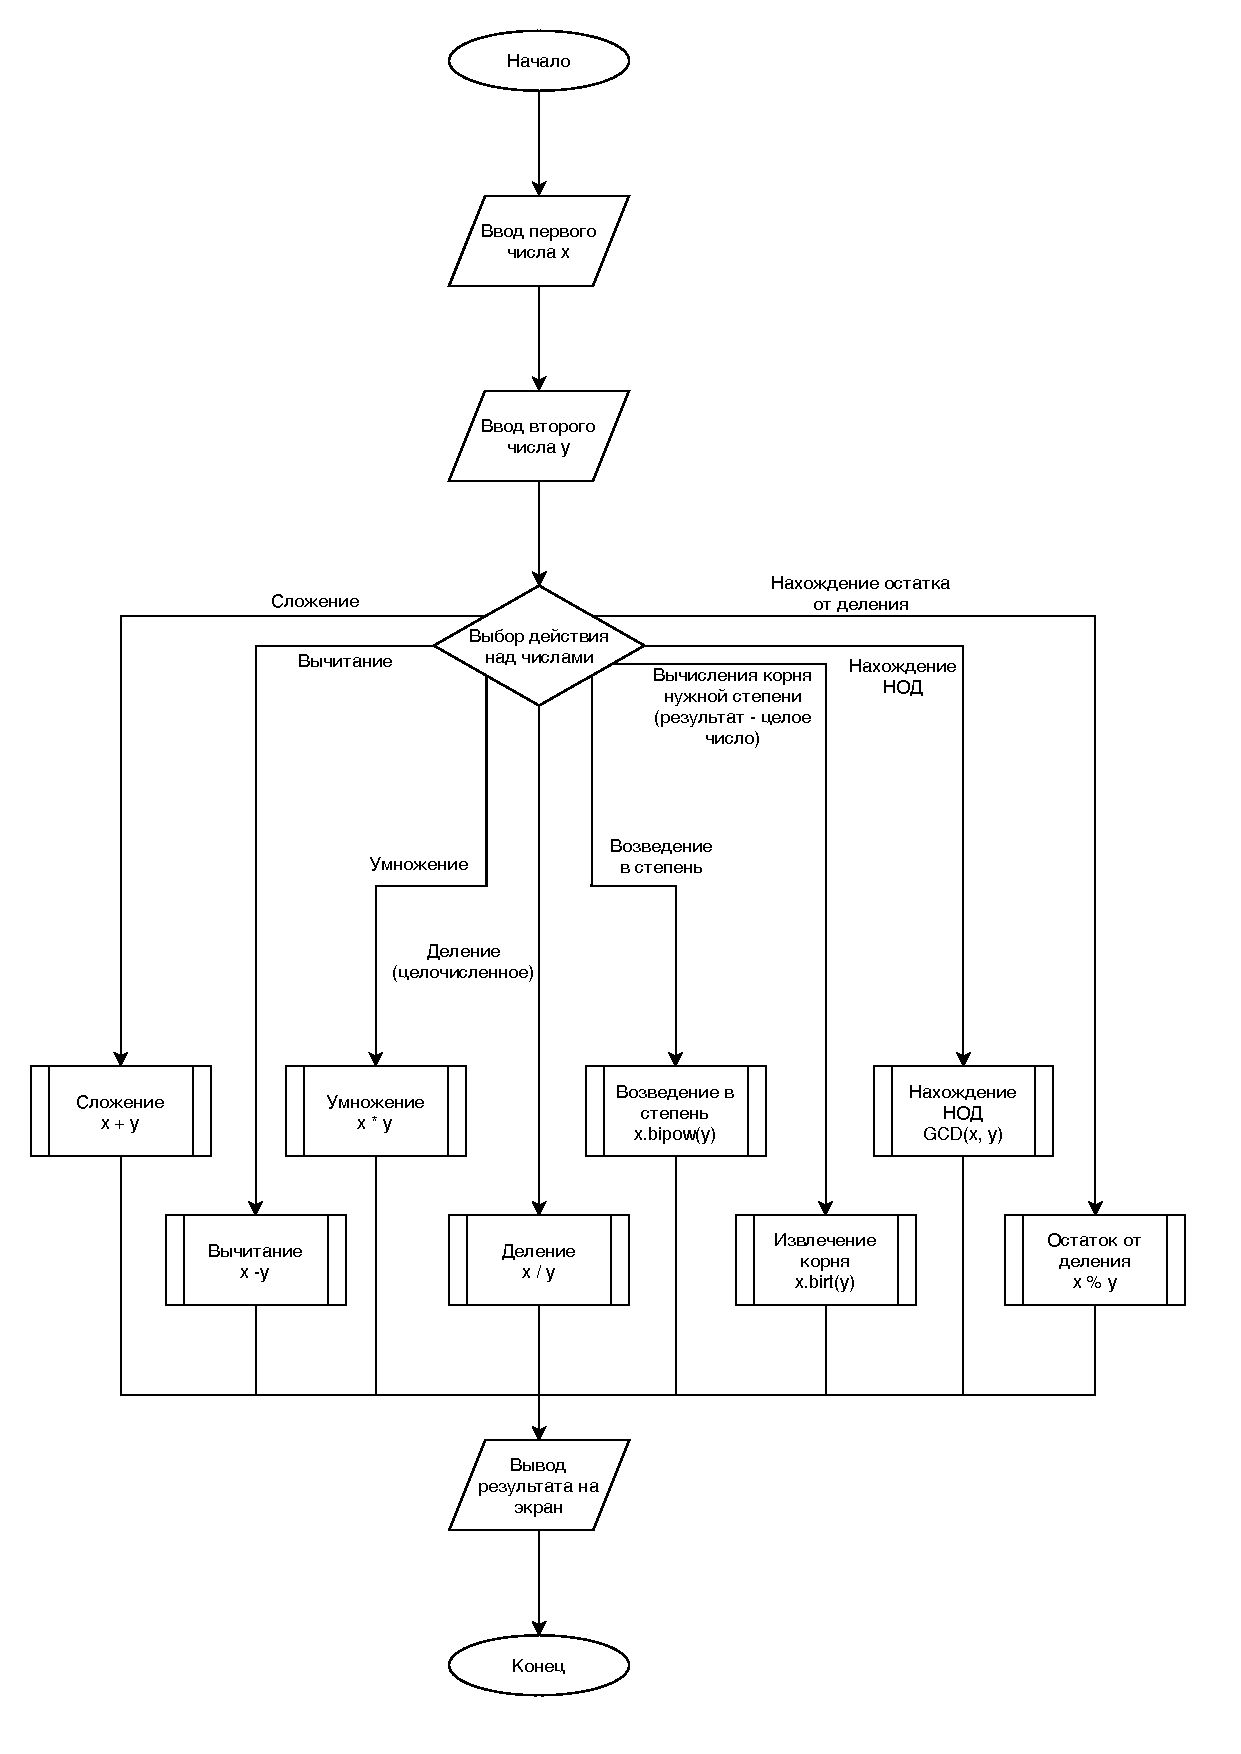
\includepdf[pages=-]{./Flowchart.pdf}
